\newpage
\hypertarget{static:classes tex}{}
\subsection{Declaring classes and attributes}
\texHeader

\begin{itemize}

\item[$\blacktriangleright$] Right click your \texttt{LearningBoxLanguage} model and create your first EClass by navigating to ``New/EClass.'' Name it
\texttt{Box}.

\vspace{0.5cm}

\item[$\blacktriangleright$] The class editor should automatically open. Let's add the first two EAttributes of our program, \texttt{name} and
\texttt{stringRep}. eMoflon offers type completion templates to help you with this task. Go to an empty line and press \texttt{ctrl + space}. You'll be provided
with a short list of suggestions (Fig.~\ref{fig:typeCompTempl}). The first four items are related to method control flow, so select \texttt{attribute} near
the bottom, and create \texttt{name} of type \texttt{EString}.

\vspace{0.5cm}

\begin{figure}[htbp]
	\centering
  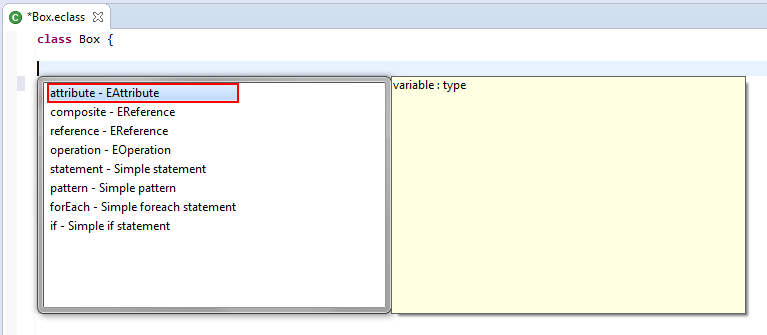
\includegraphics[width=0.6\textwidth]{eclipse_typeCompletionTemplates}
	\caption{eMoflon's type completion}
	\label{fig:typeCompTempl}
\end{figure} 

\vspace{0.5cm}

\item[$\blacktriangleright$] Type completion also supports you by suggesting a list of types. Start to create a second attribute, \texttt{stringRep}, but
stop after typing the \texttt{`:'} operator and press the hotkeys. The pop-up list provides a list of all types currently available (Fig.~\ref{fig:typeCompTypes}) in
both your metamodel, and eMoflon's standard metamodel that's included in every new project.

\vspace{0.5cm}

\item[$\blacktriangleright$] Your workspace should now resemble (Fig.~\ref{fig:boxDeclaration}).

\newpage

\begin{figure}[htbp]
	\centering
  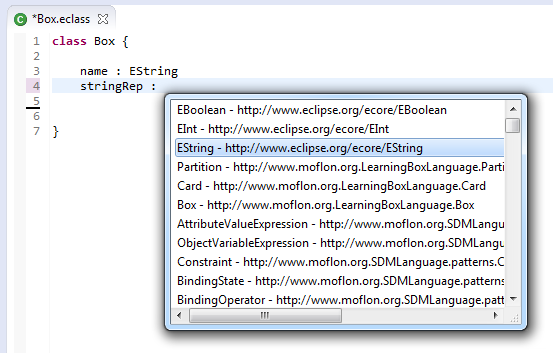
\includegraphics[width=0.6\textwidth]{eclipse_typeCompletionTypes}
	\caption{Object type suggestions for \texttt{stringRep}}
	\label{fig:typeCompTypes}
\end{figure} 

\vspace{0.5cm}

\begin{figure}[htbp]
	\centering
  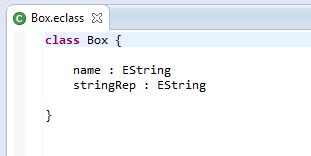
\includegraphics[width=0.5\textwidth]{eclipse_classBoxDeclaration}
	\caption{Newly created \texttt{Box} EClass}
	\label{fig:boxDeclaration}
\end{figure} 
\FloatBarrier

\vspace{0.5cm}

\item[$\blacktriangleright$] Now create two empty EClasses in your model, \texttt{Partition} and \texttt{Card}.

\vspace{0.5cm}

\item[$\blacktriangleright$] In \texttt{Partition}, add two \texttt{EInt} attributes, \texttt{index} and \texttt{partitionSize}.

\vspace{0.5cm}

\item[$\blacktriangleright$] In \texttt{Card}, create three \texttt{EString} attributes, \texttt{back}, \texttt{face} , and \texttt{partitionHistory}.

\vspace{0.5cm}

\item[$\blacktriangleright$] If you've done everything correctly, your workspace should now resemble Fig.~\ref{fig:workspaceClassAttributes}.

\begin{figure}[htbp]
	\centering
  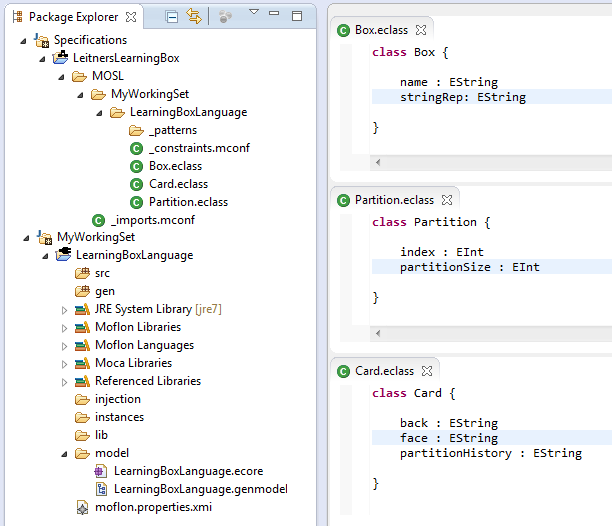
\includegraphics[width=1.0\textwidth]{eclipse_workspaceTexClassAttributes}
	\caption{Declaration of all EClasses and attributes}
	\label{fig:workspaceClassAttributes}
\end{figure} 

\vspace{0.5cm}

\item[$\blacktriangleright$] That's it for declaring class attributes! Feel free to build your project again and view the changes in the \texttt{.ecore}
mode, and the generated files in ``gen" and ``src." On a final note, while some languages (such as Java) allow the declaration of several small classes (such as
these three) in the same file, when tooling with eMolfon, we keep them separated. Don't worry - we'll explain this later in the handbook. As for now, continue
to the next section to start creating references between these EClasses.

% \fancyfoot[R]{$\triangleright$ \hyperlink{static:references splash}{Next}}

\end{itemize}
